\documentclass[11pt,letterpaper]{article}
\usepackage[top=3cm, bottom=2cm, left=2cm, right=2cm, columnsep=20pt]{geometry}
\usepackage{pdfpages}
\usepackage{graphicx}
\usepackage{etoolbox}
\apptocmd{\sloppy}{\hbadness 10000\relax}{}{}
% \usepackage[numbers]{natbib}
\usepackage[T1]{fontenc}
\usepackage{ragged2e}
\usepackage[french]{babel}
\usepackage{listings}
\usepackage{color}
\usepackage{soul}
\usepackage[utf8]{inputenc}
\usepackage[export]{adjustbox}
\usepackage{caption}
\usepackage{amsmath}
\usepackage{amssymb}
\usepackage{float}
\usepackage{csquotes}
\usepackage{fancyhdr}
\usepackage{wallpaper}
\usepackage{siunitx}
\usepackage[indent]{parskip}
\usepackage{textcomp}
\usepackage{gensymb}
\usepackage{multirow}
\usepackage[hidelinks]{hyperref}
\usepackage{abstract}
\renewcommand{\abstractnamefont}{\normalfont\bfseries}
\renewcommand{\abstracttextfont}{\normalfont\itshape}
\usepackage{titlesec}
\titleformat{\section}{\large\bfseries}{\thesection}{1em}{}
\titleformat{\subsection}{\normalsize\bfseries}{\thesubsection}{1em}{}
\titleformat{\subsubsection}{\normalsize\bfseries}{\thesubsubsection}{1em}{}

\usepackage{xcolor}
\definecolor{codegreen}{rgb}{0,0.6,0}
\definecolor{codegray}{rgb}{0.5,0.5,0.5}
\definecolor{codepurple}{rgb}{0.58,0,0.82}
\definecolor{backcolour}{rgb}{0.95,0.95,0.92}
\lstdefinestyle{mystyle}{
    backgroundcolor=\color{backcolour},   
    commentstyle=\color{codegreen},
    keywordstyle=\color{magenta},
    numberstyle=\tiny\color{codegray},
    stringstyle=\color{codepurple},
    basicstyle=\ttfamily\footnotesize,
    breakatwhitespace=false,         
    breaklines=true,                 
    captionpos=b,                    
    keepspaces=true,                 
    numbers=left,                    
    numbersep=5pt,                  
    showspaces=false,                
    showstringspaces=false,
    showtabs=false,                  
    tabsize=2
}
\lstset{style=mystyle}

\usepackage[most]{tcolorbox}
\newtcolorbox{note}[1][]{
  enhanced jigsaw,
  borderline west={2pt}{0pt}{black},
  sharp corners,
  boxrule=0pt, 
  fonttitle={\large\bfseries},
  coltitle={black},
  title={Note:\ },
  attach title to upper,
  #1
}

%----------------------------------------------------

\setlength{\parindent}{0pt}
\DeclareCaptionLabelFormat{mycaptionlabel}{#1 #2}
\captionsetup[figure]{labelsep=colon}
\captionsetup{labelformat=mycaptionlabel}
\captionsetup[figure]{name={Figure }}
\newcommand{\inlinecode}{\normalfont\texttt}
\usepackage{enumitem}
\setlist[itemize]{label=\textbullet}

\begin{document}
\begin{titlepage}
\center

\begin{figure}
    \ThisULCornerWallPaper{.4}{Polytechnique_signature-RGB-gauche_FR.png}
\end{figure}
\vspace*{2 cm}

\textsc{\Large \textbf{PHS2223 --} Introduction à l'optique moderne}\\[0.5cm]
\large{\textbf{Équipe : 04}}\\[1.5cm]

\rule{\linewidth}{0.5mm} \\[0.5cm]
\Large{\textbf{Expérience 4}} \\[0.2cm]
\text{Filtrage spatial}\\
\rule{\linewidth}{0.2mm} \\[2.3cm]

\large{\textbf{Présenté à}\\
  Guillaume Sheehy\\
  Esmat Zamani\\[2.5cm]
  \textbf{Par :}\\
  Émile \textbf{Guertin-Picard} (2208363)\\
  Laura-Li \textbf{Gilbert} (2204234)\\
  Tom \textbf{Dessauvages} (2133573)\\[3cm]}

\large{\today\\
Département de Génie Physique\\
Polytechnique Montréal\\}

\end{titlepage}

%----------------------------------------------------

\tableofcontents
\pagenumbering{roman}
\newpage

\pagestyle{fancy}
\setlength{\headheight}{14pt}
\renewcommand{\headrulewidth}{0pt}
\fancyfoot[R]{\thepage}

\pagestyle{fancy}
\fancyhf{}
\renewcommand{\headrulewidth}{1pt}
\fancyhead[L]{\textbf{PHS2223}}
\fancyhead[C]{Rapport final}
\fancyhead[R]{\today}
\fancyfoot[R]{\thepage}

\pagenumbering{arabic}
\setcounter{page}{1}

%----------------------------------------------------

\section{Résultats}

\subsection{Cibles de résolution}

\begin{figure}[H]
  \centering
  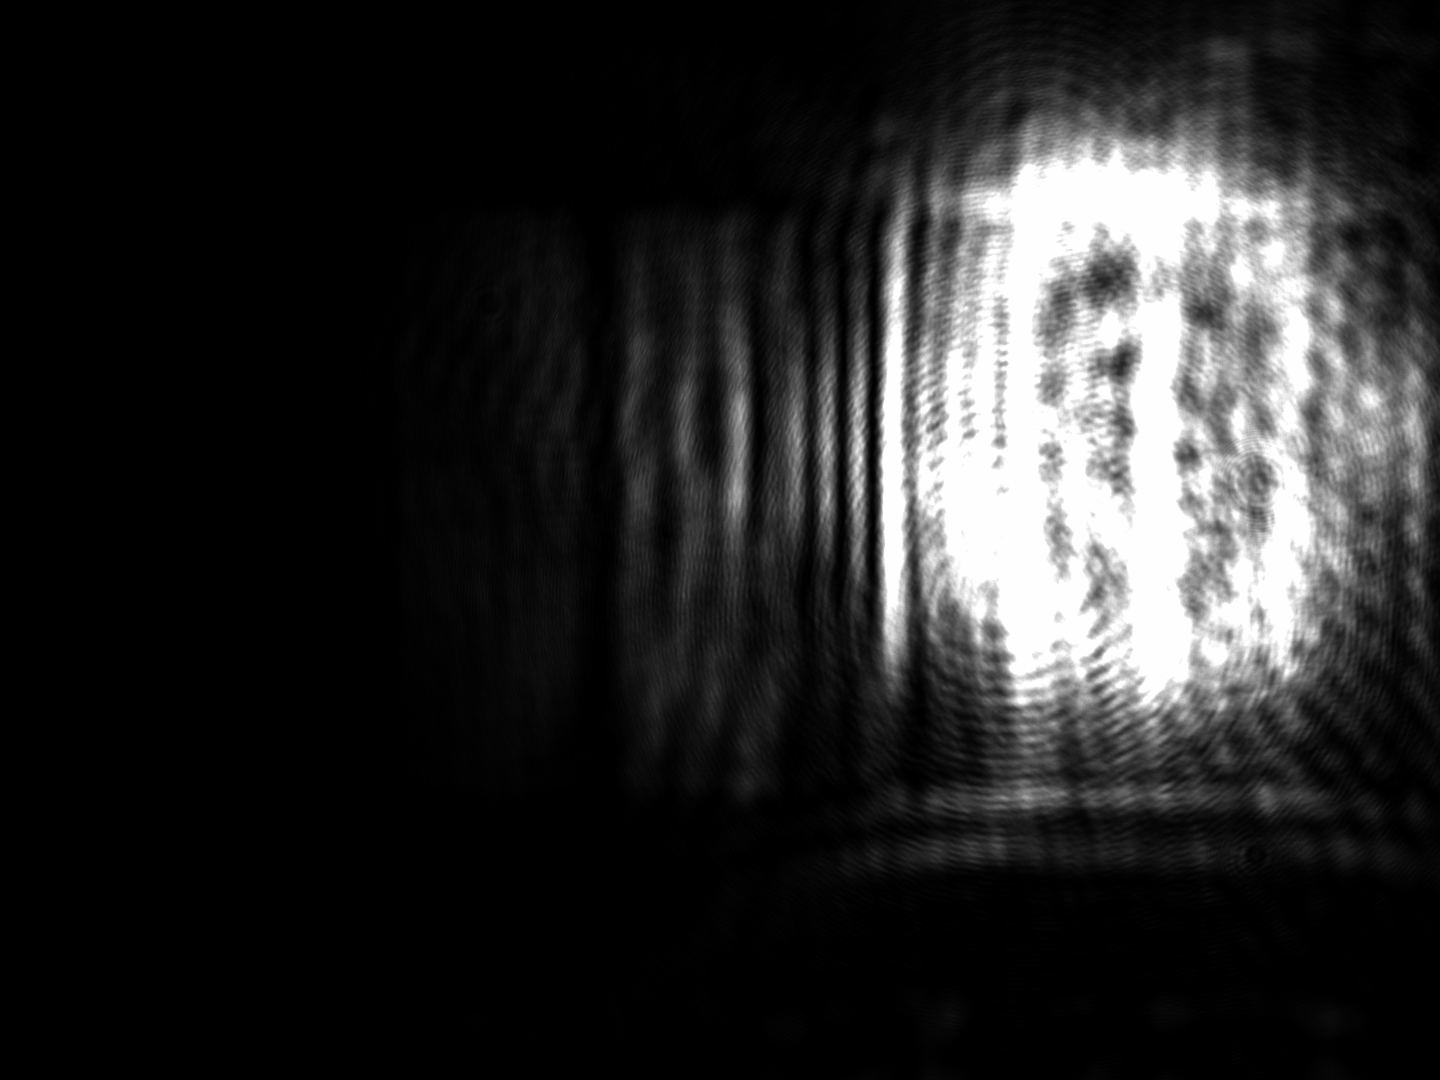
\includegraphics[scale=0.3]{cible_d1.2_1-7.png}
  \caption{}
  \label{}
\end{figure}


\subsection{Marvin}


\section{Discussion}

\subsection{Question 1}
Pour trouver la fréquence de coupure de l'iris selon les paramètres physiques de l'expérience, les deux équations de fréquences spatiales peuvent être utilisées. L'équation pour la fréquence spatiale en $x$ est donnée par :
\begin{equation}
  f_{x}=\frac{x}{\lambda f}
  \label{eqfx}
\end{equation}
Et celle en $y$ est donnée par :
\begin{equation}
  f_{y}=\frac{y}{\lambda f}
  \label{eqfy}
\end{equation}
Où $\lambda$ est la longueur d'onde de la lumière, et $f$ est la longueur focale de la lentille utilisée. Puisque le filtre est de forme circulaire, il est possible de modéliser la fréquence de coupure à l'aide de l'équation d'un cercle, soit la suivante :
\begin{equation}
  x^{2}+y^{2}=r^{2}
  \label{eqcercle}
\end{equation}
Où $r$ correspond au rayon de l'iris. Donc, en isolant les variables $x$ et $y$ dans les équations \ref{eqfx} et \ref{eqfy}, et en remplaçant dans l'équation ci-dessus (Annexe), le résultat suivant est obtenu :
\begin{equation}
  f_{c}=\frac{r}{\lambda f}=\frac{d}{2\lambda f}
  \label{eqfc}
\end{equation}
Ainsi, la fréquence de coupure de l'iris selon les paramètres physiques est donnée par l'équation ci-dessus.

\textcolor{red}{RÉSULTATS COHÉRENTS AVEC THEO?}

\subsection{Question 2}

\section{Conclusion}

\newpage\section*{Annexe}
Avec les équations $f_{x}$ et $f_{y}$, les variables $x$ et $y$ sont isolées, permettant d'obtenir les équations suivantes :
\begin{align*}
  x&=f_{x}\lambda f & y&=f_{y}\lambda f \\
\end{align*}
En remplaçant dans l'équation \ref{eqcercle}, le résultat suivant est obtenu.
\begin{align*}
  (f_{x}\lambda f)^{2}+(f_{y}\lambda f)^{2}&=r^{2} \\
  f_{x}^{2}\lambda^{2}f^{2}+f_{y}^{2}\lambda^{2}f^{2}&=r^{2} \\
  \lambda^{2}f^{2}(f_{x}^{2}+f_{y}^{2})&=r^{2} \\
\end{align*}
En réarrangeant les termes, le résultat suivant est obtenu.
\begin{equation*}
  (f_{x}^{2}+f_{y}^{2})=\frac{r^{2}}{\lambda^{2}f^{2}}
\end{equation*}
Les deux fréquences spatiales $f_{x}$ et $f_{y}$ correspondent à la fréquence recherchée, ainsi l'équation mène à celle \ref{eqfc}, soit :
\begin{equation*}
  f_{c}=\frac{r}{\lambda f}=\frac{d}{2\lambda f}
\end{equation*} 

\clearpage

% \bibliographystyle{unsrtnat}
% \bibliography{My_Library}

\end{document}
